\subsection{Individuazione target d'utenti}
    \begin{flushleft}
        La conoscenza dell'utente finale è di importanza fondamentale per chi progetta sistemi software di questo tipo. La grande diversità degli esseri umani
        fa sì che, anche considerando compiti e contesti d'uso simili, un oggetto potrebbe risultare usabile per un certo utente e
        del tutto inusabile per un altro.\\
        Sicuramente, in base alle richieste del committente abbiamo subito individuato 4 principali categorie di utenti utilizzatori dell'app:
        \vspace{0.5cm}
       
        \textbf{Admin:} Amministratore e proprietario del ristorante. Una persona che deve avere tutto sotto controllo, può gestire le sue attività nonchè i 
        dipendenti che ne fanno parte, aggiungerne di nuovi e talvolta, purtroppo, eliminarli.
        \vspace{1cm}

        \textbf{Supervisore:} Dopo l'amministratore, è, nella "gerarchia" da noi definita, la seconda persona con più funzioni disponibili in-app. 
        Anch'esso dispone di una dashboard completa sullo stile dell'admin.
        \vspace{1cm}

        \textbf{Cameriere/Addetto sala:} Senza la figura del cameriere un'attività di ristorazione non va avanti. Sappiamo quant'è importante fornire a questi ultimi
        un applicativo funzionale, facile da usare e da apprendere: per questo la sua interfaccia è ottimizzata per un palmare o smartphone compatto.
        \vspace{1cm}


        \textbf{Addetto Cucina:} Riceve tutti gli ordini dai camerieri e li inoltra alla cucina. Anche lui dispone di un'interfaccia semplice e dinamica che perfettamente si adatta al suo ruolo nell'attività.
        \vspace{0.5cm}        
        
        Tutto ciò è reso possibile da uno sviluppo che va incontro alle esigenze dei diversi utenti. La nostra interfaccia riconosce il tipo di utente che logga e cambia
        in base alle sue esigenze. 

    \end{flushleft}


    \begin{figure}[H]
        \centering
        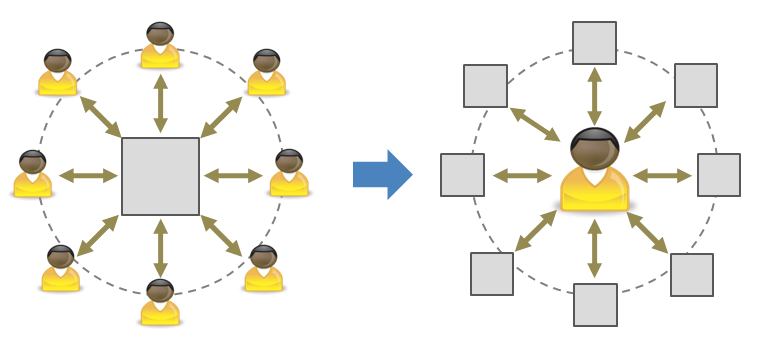
\includegraphics[scale=0.5]{assets/immagini varie/target utenti.png}
        \caption*{\textbf{Figura}: Da una visione centrata sul sistema a una visione centrata sull’utente}\label{fig:target_utenti}
    \end{figure}